\section {Backend}

The client agreed on having an Erlang version of a NetInf Name Resolution Server(NetInf NRS).  Our backend product implements the current draft NetInf Protocol in a distributed and purely functional language. The product promises a high level of scalability and fault-tolerance. The client initially asked for only the NRS as a product however the backend team was able to complete the initial product in a timely manner, allowing for applications of this network technology to be explored. 


\subsection {Erlang NetInf Name Resolution Server}
The first of the two deliverables from the backend team to the client. The Erlang NetInf Name Resolution Server(NetInf NRS) provides a new way to organize and retrieve data on the internet. Based on a inital NetInf NRS protocol draft from development teams such as SAIL and Ericsson Research. This product allows for flexibility and extension of the existing protocol.

Erlang's concept of modularization allowed the team to break up the NRS functionality into distinctive convergence layers, real-time database switching, and even allow for a proof of concept video streaming client/protocol. 

\subsection{NetInf Video Streaming Client/Protocol}

The last of the deliverables from the backend team. The client asked for a proof of concept of a streaming protocol and client which lies on top of the Erlang NetInf NRS technology. The streaming protocol is a completely new addition to the NetInf draft. Our team came up with a way to utilize the code and transporting mechanism of the first product in order to stream video content, along with the protocol outlined below we have been able to create a http interface 'client' which allows you to see the streaming protocol in action as well access the NRS functionality. This particular product was not specified in the initial conversations with the client in September, but added late in the development cycle and is not meant to be a complete product.

\subsubsection{First Implementation}
In addition to normal NRS functionality, to get transfer of chunks to work a http transfer-dispatcher had to be implemented. The streaming works by clients subscribing to a stream from a specific NRS and with an constant interval  asking that NRS where to find these chunks. All the chunks are transferred via the transfer-dispatcher.
The playback of the video chunks are done by polling the local NRS, this implies that every client has its own NetInf node running. See figure \ref{fig:stream-seqorgmod}. The benefit of using this approach is that only one NDO containing the filename has to be published. The receiver can then derive the chunks locations, by appending the chunk number to the end of the locators provided in the filename NDO.

\begin{figure}[h!]
	\centering
		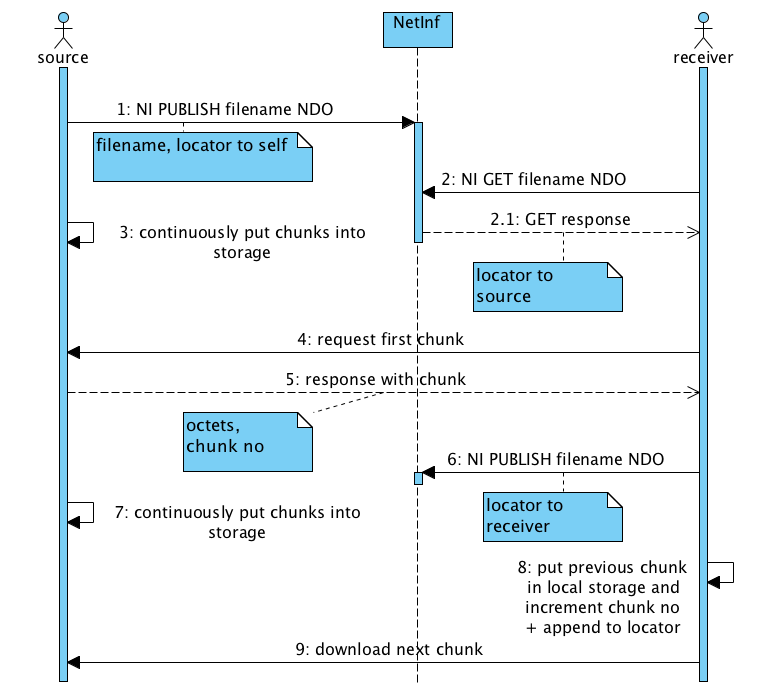
\includegraphics[width=0.75\textwidth]{./img/sequence_diagram_streaming_orgmod.png}
    	\caption{Original/Modified Chunked Data Transfer}
	\label{fig:stream-seqorgmod}
\end{figure}

\subsubsection{Modified NetInf Streaming}
Due to a request from the client a more true NetInf implementation of streaming was implemented. Instead of using the transfer-dispatcher between the client nodes a workaround was added that disabled content validation, this resulted in it being possible to fetch chunks via NetInf messages. The polling logic is still the same as first implementation, seen in figure \ref{fig:stream-seqorgmod}. Instead of using ordinary http locators, the receiver need to modify the \textit{NetInf GET requests} to get the chunks, this is done by replacing the hash algorithm with the custom hash name \textit{demo}. For example to get the first chunk of \textit{ni:///sha-256;abc}, the request should contain \textit{ni:///demo;abc1}. The http transfer-dispatcher is still used to transfer the chunks to the HTML-interface.

\subsubsection{Pure NetInf Streaming}
To be able to evaluate the modified NetInf streaming another implementation was added, this implementation uses NetInf searches and gets for chunks. See Figure~\ref{fig:stream-seq-pure}. In this implementation the stream source needs to publish each chunk to the NRS, needs to put the stream name and stream chunk number in the NDO metadata. The receiver then needs to search for each chunk to find it. 

\begin{figure}[h!]
	\centering
		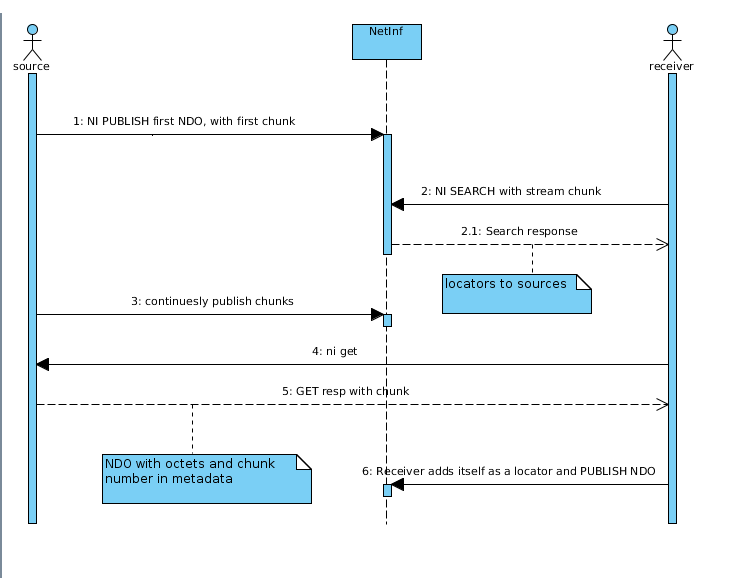
\includegraphics[width=0.75\textwidth]{./img/sequence_diagram_pure_streaming.png}
    	\caption{Chunked Data Transfer With Pure NetInf}
	\label{fig:stream-seq-pure}
\end{figure}

\subsubsection{Streaming Frontend}
To merge the chunks, a simple HTML5 frontend was added. HTML was the choice  to make the player platform independent.
In both implementations the player starts a JavaScript that continuously polls the local NetInf node for the chunks through the http dispatcher.
The difference is that the pure NetInf player, uses the NRS search to build the playlist, while the modified NetInf version just increase the chunk number.
